\section{\textcolor[HTML]{D32F2F}{Axure}}
Versjon 2 av designet ble laget i et program kalt Axure. Dette er et verktøy for prototyping, spesifisering og diagrammer. Her kan man planlegge en prototype, og lage en troverdig app. Det gjør det mulig for gruppen å teste den faktiske opplevelsen av bruk på testpersonene. Modellen blir interaktiv og responderer på klikk. Axure-modellen er med andre ord langt mer avansert enn den forrige prototypen som ble testet med Wizard-of-Oz.

\subsection{Designbeslutninger}
I denne versjonen ble tilbakemeldingene fra brukertesten tatt med. Det ble gjort flere endringer i designet, blant annet ble det lagt inn deleknapp for ønskelister slik at brukeren kan dele direkte på Facebook eller e-post. Boksene i appen ble også endret fra å ha bokser med runde hjørner til å ha firkantede hjørner. Dette ble gjort for å få et pent og gjennomgående design, ikke fordi det hadde noen funksjon ellers i appen. Det siste som ble endret var handlelisten.
\\\\
Å ha en meny i produktet ble fort avgjort som nødvendig for en god brukeropplevelse. En meny skal gjerne vise innholdet på en strukturert måte, slik at brukeren skal kunne velge mellom et sett med valg \cite[s.~166]{preece}. Menyer i interface er gjerne plassert i topp- eller bunnlinjen av skjermen, eller langs venstre side. Det er mange måter å gjøre dette på, og eksempler er lister, drop-down, pop-up, kontekstuelle, ekspanderende og scrolling. Gruppen valgte å gå for en enkel meny, siden det er få sider i designet og målet var at appen skulle være enklest mulig.
\\\\
Farger er også viktig for å få en ideell brukeropplevelse. Farger i seg selv signaliserer mye til brukeren, men også valg av farger å komponere er avgjørende. Å lese en grønn tekst på rød bakgrunn er slitsomt for øynene, og det samme er turkis på grå bakgrunn\cite{esthetics}. Det optimale er svart på hvitt for god lesbarhet, men det velges ofte farger for å sprite opp designet. Da er det vanlig å lage en fargepalett, hvor de samme fargene går gjennom i hele designet. Siden Sirkus shopping har en rød profil, valgte gruppen å videreføre denne i appen.

\begin{figure}[H]
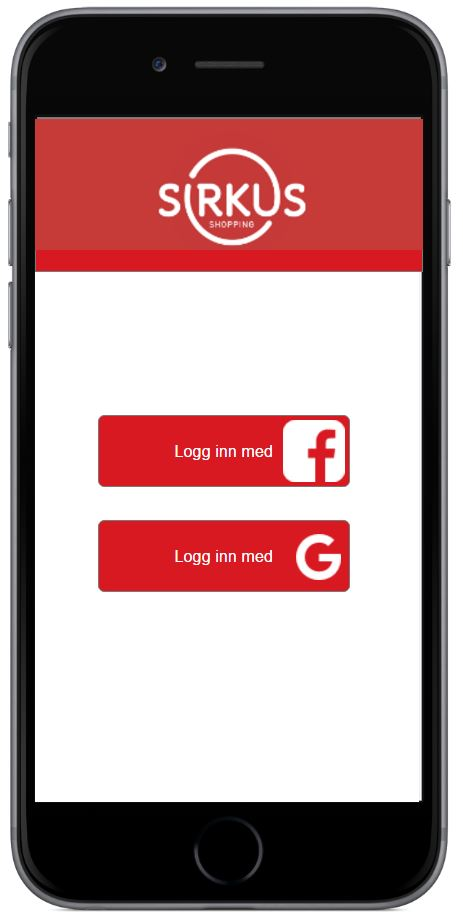
\includegraphics[scale=0.55]{images/axurebilder/login}
\centering %centering the image
\caption{Logge inn}
\label{fig:login}
\end{figure}

\begin{figure}[H]
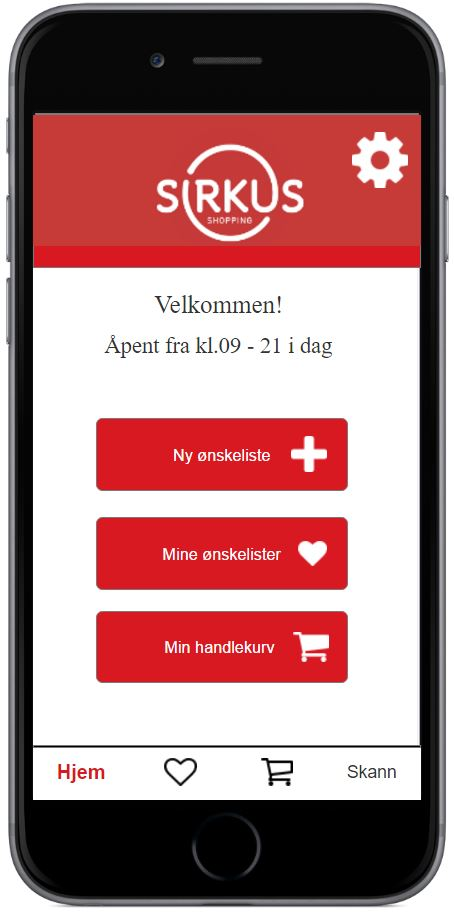
\includegraphics[scale=0.55]{images/axurebilder/hjem}
\centering %centering the image
\caption{Hjem}
\label{fig:hjem}
\end{figure}

\begin{figure}[H]
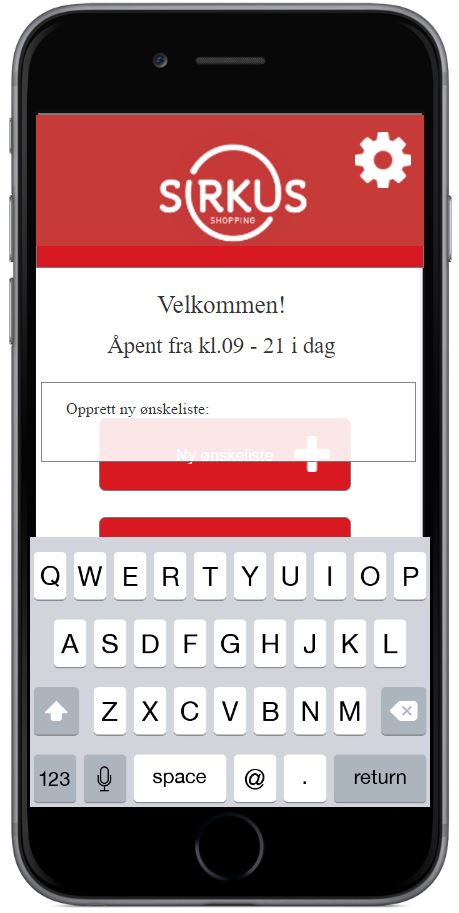
\includegraphics[scale=0.55]{images/axurebilder/opprett_onskeliste_hjem}
\centering %centering the image
\caption{Opprett ønskeliste startside}
\label{fig:opprett_onskeliste_hjem}
\end{figure}

\begin{figure}[H]
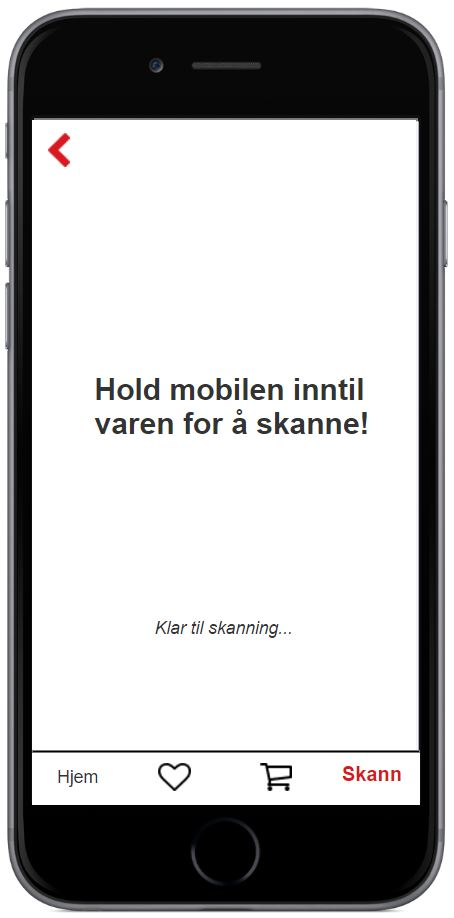
\includegraphics[scale=0.55]{images/axurebilder/skann}
\centering %centering the image
\caption{Skann produkt}
\label{fig:skann}
\end{figure}

\begin{figure}[H]
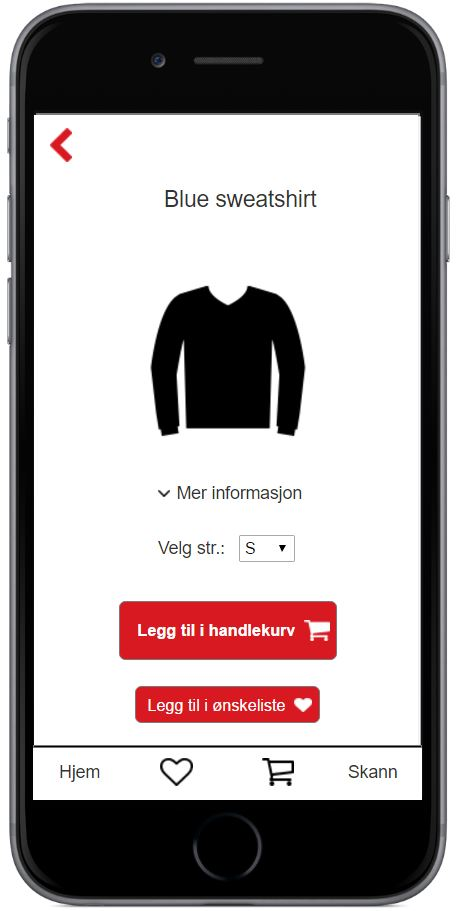
\includegraphics[scale=0.55]{images/axurebilder/genser}
\centering %centering the image
\caption{Produkt}
\label{fig:genser}
\end{figure}

\begin{figure}[H]
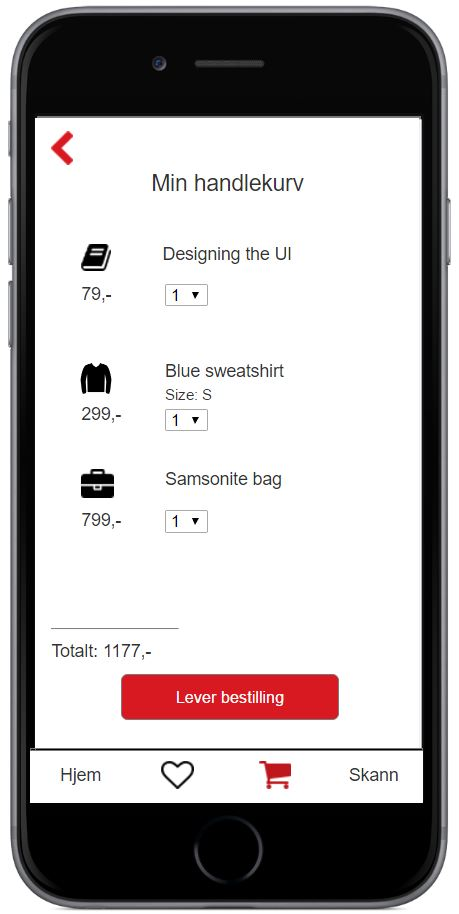
\includegraphics[scale=0.55]{images/axurebilder/handlekurv}
\centering %centering the image
\caption{Handlekurv}
\label{fig:handlekurv}
\end{figure}

\begin{figure}[H]
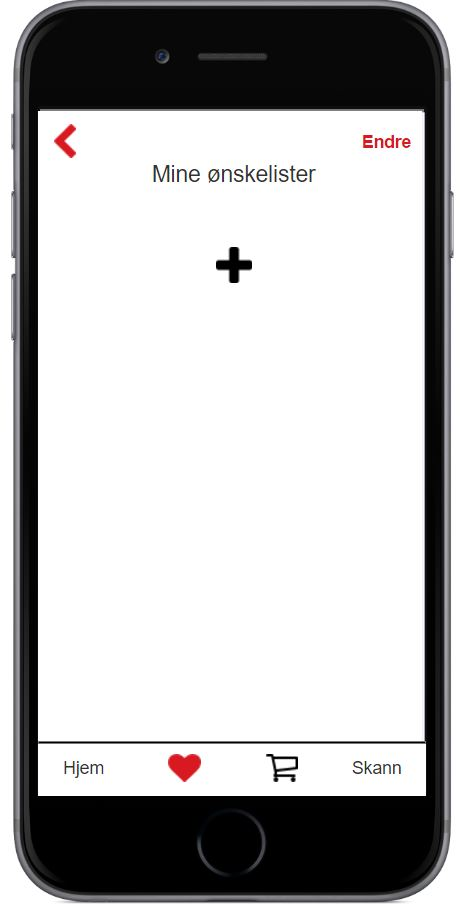
\includegraphics[scale=0.55]{images/axurebilder/mine_onskelister_tom}
\centering %centering the image
\caption{Tom oversikt over mine ønskelister}
\label{fig:mine_onskelister_tom}
\end{figure}

\begin{figure}[H]
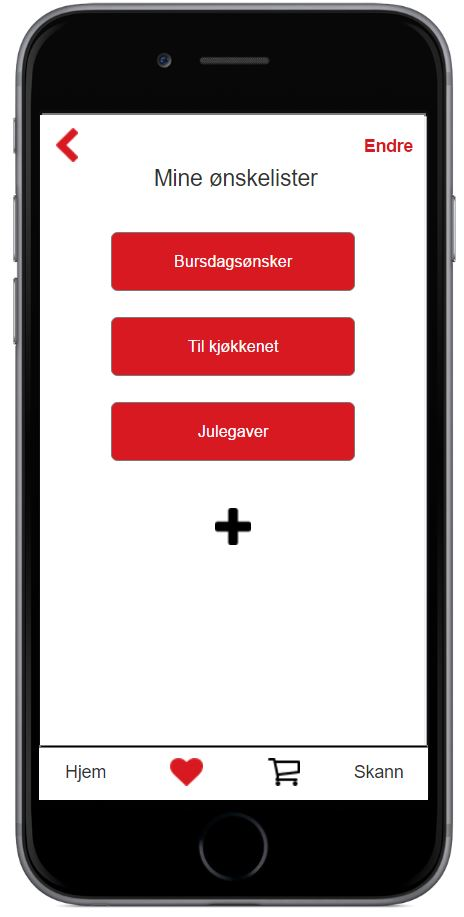
\includegraphics[scale=0.55]{images/axurebilder/mine_onskelister_2}
\centering %centering the image
\caption{Mine ønskelister}
\label{fig:mine_onskelister_2}
\end{figure}

\begin{figure}[H]
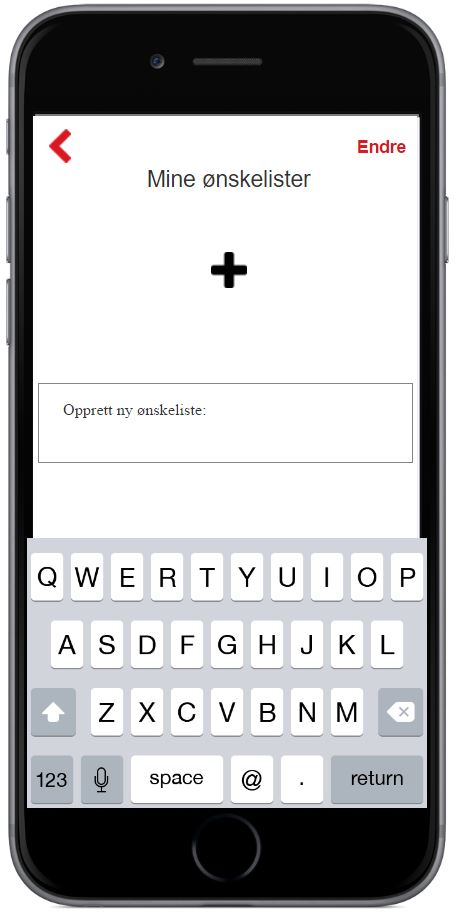
\includegraphics[scale=0.55]{images/axurebilder/opprett_onskeliste_2}
\centering %centering the image
\caption{Opprett ønskeliste}
\label{fig:opprett_onskeliste_2}
\end{figure}

\begin{figure}[H]
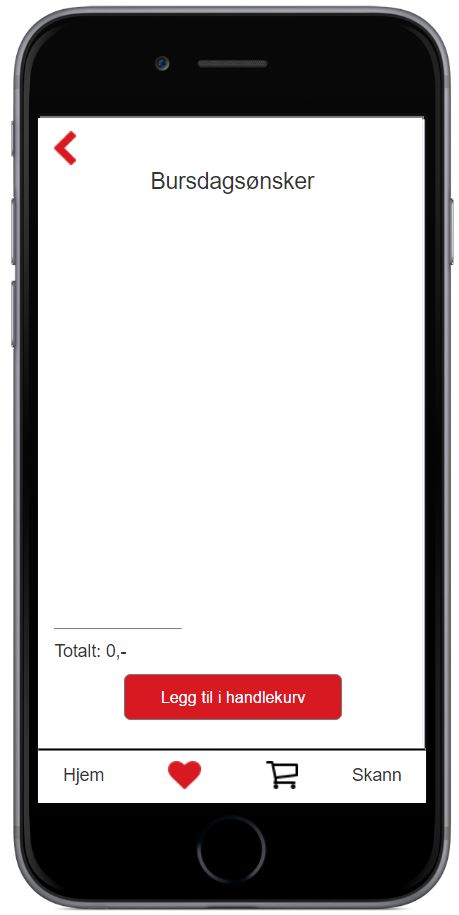
\includegraphics[scale=0.55]{images/axurebilder/bursdagsonsker_tom}
\centering %centering the image
\caption{Tom liste for bursdagsønsker}
\label{fig:bursdagsonsker_tom}
\end{figure}

\begin{figure}[H]
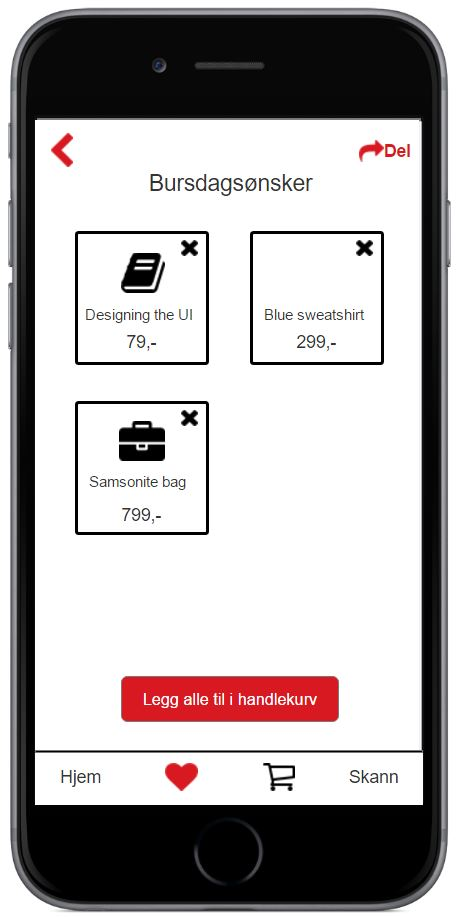
\includegraphics[scale=0.55]{images/axurebilder/bursdagsonsker}
\centering %centering the image
\caption{Liste for bursdagsønsker, med innhold}
\label{fig:bursdagsonsker}
\end{figure}

\begin{figure}[H]
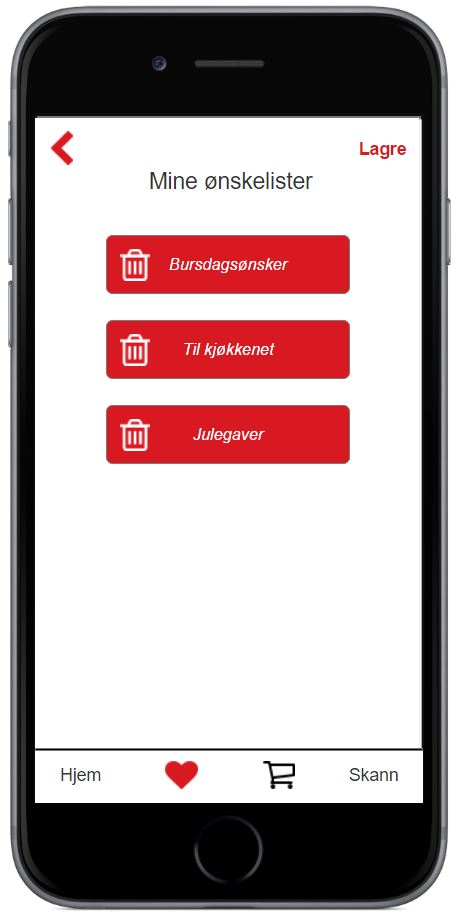
\includegraphics[scale=0.55]{images/axurebilder/endre_mine_onskelister_2}
\centering %centering the image
\caption{Endre ønskelister}
\label{fig:endre_mine_onskelister_2}
\end{figure}

\begin{figure}[H]
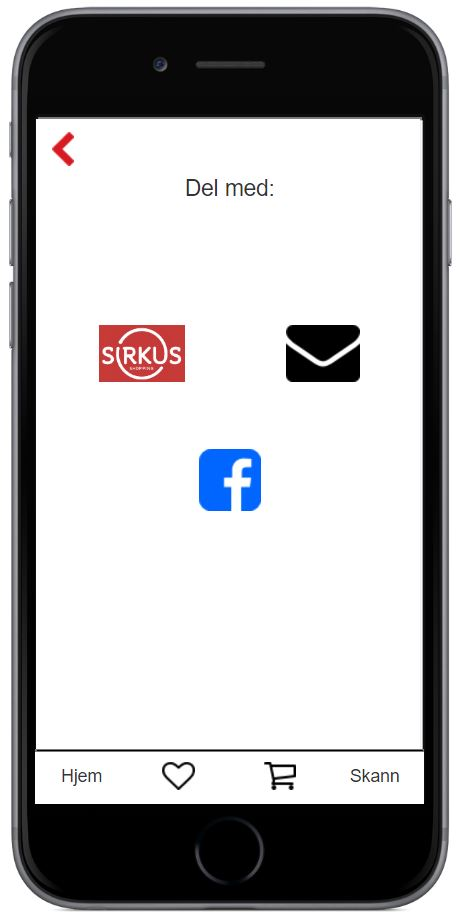
\includegraphics[scale=0.55]{images/axurebilder/del}
\centering %centering the image
\caption{Del liste}
\label{fig:del}
\end{figure}

\begin{figure}[H]
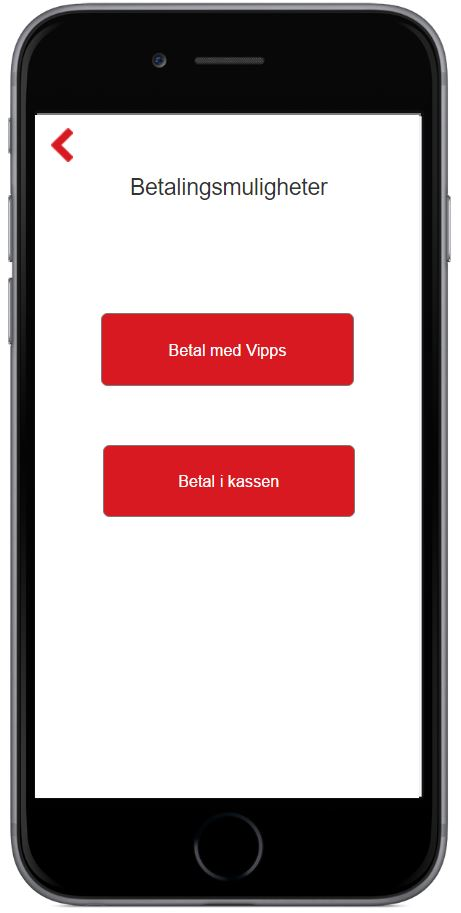
\includegraphics[scale=0.55]{images/axurebilder/betalingsmuligheter}
\centering %centering the image
\caption{Betalingsmuligheter i app}
\label{fig:betalingsmuligheter}
\end{figure}

\begin{figure}[H]
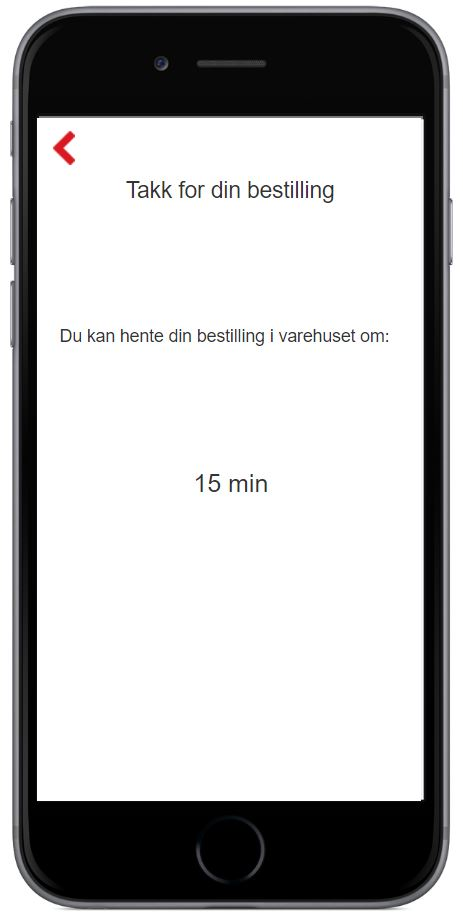
\includegraphics[scale=0.55]{images/axurebilder/hent_varer}
\centering %centering the image
\caption{Hent varer}
\label{fig:hent_varer}
\end{figure}

%flytdiagram

\subsection{Brukertest}
Da det skulle brukertestes gang nummer to, var det blitt laget en prototype med Axure. Denne prototypen lignet mye på det gruppen så for seg som det ferdige produktet, og denne brukertesten ble da av typen high-fidelity. Det vil si at den ligner mye på det ferdige produktet, og har flere funksjonaliteter enn en low-fidelity-prototype \cite[s.~391]{preece}. Å teste med high-fidelity har mange fordeler, siden det gir brukeren en nær opplevelse av hvordan det ferdige produktet vil se ut, men har også store kostnader. Det krever langt mer tid å utvikle en Axure-prototype enn en prototype i papir, slik gruppen brukte i Wizard-of-Oz-testen.

\subsubsection{Testprosedyre}
Brukertesten av Axure-prototypen ble gjort på lab hvor det ble brukt eyetracking. Dette er et kamera som er festet på undersiden av skjermen, som detekterer hvor øynene ser. Før testen starter kalibrerer man programmet mot øynene, slik at man er sikker på at punktene brukeren ser på blir registrert. Deretter setter man kameraet på opptak, og vil da kunne se hvor brukeren ser til enhver tid, samt hvordan øynene forflytter seg over skjermen.
\\\\
Testpersonen som ble brukt i eyetracking-testen var Hege Louise Borge, en student ved masterstudiet i informatikk på NTNU. 
\\\\\
Testspørsmålene som ble brukt under brukertesten var relativt like de som ble stilt i den forrige brukertesten. Dette ble gjort med hensikt, fordi det da er lettere å sammenligne resultatene. Noen endringer måtte likevel gjøres, siden appen hadde fått noen endrede funksjoner. Testspørsmålene er listet under.

\begin{enumerate}
    \item Logg inn med valgfritt innloggingsverktøy
    \item Du skal lage en oversikt over dine bursdagsønsker. Lista skal hete “bursdagsønsker”.
    \item Legg til en genser i listen over bursdagsønsker.
    \item Naviger deg tilbake til oversikten over mine ønskelister.
    \item Du er på oversikten over dine ønskelister. Naviger deg tilbake til startsiden.
    \item Genseren du har lagt i ønskelisten er i feil størrelse. Bytt størrelse.
    \item Del listen “Bursdagsønsker” med en venn. Velg selv delingsplattform.
    \item Slett ønskelisten “Julegaver”
    \item Gjennomfør et kjøp av denne genseren.
\end{enumerate}

\subsubsection{Resultat}
Den første oppgaven som ble gitt var å logge inn med et valgfritt innloggingsverktøy. Her valgte testpersonen å logge inn med Facebook, med en kommentar om at hun egentlig var litt skeptisk til å logge inn via dette. Ellers ble oppgaven løst uten problem. 
I oppgave to ble testpersonen bedt om å lage en oversikt over sine bursdagsønsker, og listen skulle hete “bursdagsønsker”. Brukeren trykket på ikonet for ny ønskeliste, skrev inn navn på listen og trykket “return” på tastaturet. Oppgaven ble løst vellykket.
\\\\
Neste oppgave var å legge til en genser i listen over bursdagsønsker. Her måtte brukeren tenke seg om før hun fant riktig løsning. Hun vurderte å trykke “legg til handlekurv” men konkluderte med at det ikke var det hun skulle gjøre. Hun trykket seg heller tilbake, og lette etter hvor det skulle gjøres. Siden det ikke ble gitt god nok informasjon i forkant av testen måtte testlederen bryte inn og minne om at produkter kan legges til ved å scanne varen. Da denne informasjonen ble påpekt hadde brukeren ingen problemer med å legge til varen i ønskelisten.
\\\\
Oppgaven var deretter å navigere seg tilbake til oversikten over ønskelister. Dette ble løst uten problem. Herfra fikk testpersonen i oppgave å navigere seg til startsiden. Hun nevner at hun både kan trykke på pil tilbake, og på huset nede i hjørnet for å komme seg tilbake. Hun velger å trykke på pilen. Oppgaven er løst.
\\\\
Neste oppgave testpersonen ble gitt var å endre størrelsen på genseren hun la til i ønskelisten. Brukeren lurer på hvilken størrelse hun skal endre til, men bestemmer seg for å bytte fra XS til M. Oppgaven er løst. 
\\\\	
Brukeren blir så bedt om å dele ønskelisten med en venn på en egenvalgt delingsplattform. Brukeren trykker på pilen i høyre hjørne og deler via Facebook. Hun får ingen respons på valget sitt, men blir fortalt at hun nå har delt listen.
\\\\
Deretter får hun oppgave i å slette ønskelisten kalt “Julegaver”. Brukeren går tilbake til oversikten over lister, og finner julegavelisten. Hun trykker på endre og sletter listen. Oppgaven er utført.
\\\\
Til slutt blir testpersonen bedt om å gjennomføre et kjøp av genseren. Hun legger genseren i handlekurven, leverer bestilling, betaler med Vipps og får beskjed om at varen kan hentes om 15 minutter.
\\\\
Etter testen tok testleder en prat med testpersonen om opplevelsen. Hun sa at noen ganger visste hun ikke hva hun skulle gjøre, men det gikk stort sett greit. Briefingen i forkant av testen ble ikke gjort godt nok, så testpersonen fikk ikke med seg det faktum at hun oppholdt seg på senteret. Ut over det mente hun at det nesten var umulig å gjøre feil i appen, siden det stort sett var to valg å velge mellom hele veien. Testlederen spurte om hva testpersonen tenkte om bruk av symboler som hjerte og handlevogn. Brukeren tok ikke i bruk disse symbolene, med argument om at de var like på listene og i menyen. Hun kunne brukt de, men savnet tekst under ikonene i menyen. Hun skjønte at hjerte betydde favoritt, siden hjerte eller stjerne ofte symboliserer dette, men tok dem likevel ikke i bruk. Hadde hun brukt appen flere ganger hadde hun nok brukt ikonene, i følge henne selv. Konklusjonen fra testpersonen var at appen var enkel og ikke hadde unødvendige funksjoner. En siste kommentar var at det kanskje var unødvendig med ønskelisteikoner på forsiden.

\subsubsection{Analyse}
Det må nevnes at å brukerteste en applikasjon for mobiltelefon på en datamaskin ikke er helt ideelt. På en smarttelefon bruker man knapper på telefonen og touch-skjerm for å navigere i appen. På en datamaskin brukes en mus, så resultatene er ikke helt korrekt. 

%Videoen som ble tatt opp under testen
